% Please do not delete!  thanks! -- zach
% !TEX root = ../../main.tex

In this section, we present the evaluations that been performed on our solutions. This including two parts: 1) methods that used to evaluate our core topic learning models LDA and Doc2Vec and 2) methods used to evaluate the whole solution as the final product. 

\subsection{Evaluating Learning Models}
The performance measure is a typical way to evaluate machine learning models. It is the measurement that will make of the predictions made by a trained model on the test dataset. Performance measures are typically specialized to the class of problem, for example in this paper, while we using LDA  to deal with NLP topic modeling, we will use likelihood score and clustering result to evaluate our LDA model.\\
Based on how to split the data into training and testing, evaluate machine learning models usually involves hold out, cross validation(CV) and leave-one-out. \\
Hold out method is a simple split of dataset, for example, 70\% of the instances are used for training the models, the rest 30\% for testing the model. In the CV method, it first involves separating the dataset into a number of equally sized groups of instances (called folds). The model is then trained on all folds exception one that was left out and the prepared model is tested on that left out fold. The process is repeated so that each fold get's an opportunity at being left out and acting as the test dataset. Finally, the performance measures are averaged across all folds to estimate the capability of the algorithm on the problem.  Leave-one-out is a special case of CV, where folds is equal to data points.\\
In our original plan, we may need CV to run our model evaluation, because our dataset is not large enough and the computational difficult is not critical. But with using only stackoverflow data, we have plenty of dataset. So the decision is using hold out method. We tested our models using different size of dataset. 

\paragraph{Dataset Description} 
Ultimately, we plan to use actual open source books as our primary dataset, which including over 100 books in computer science discipline. As our work went through, we plan to use some other dataset that have pre-labeled topics to train our models as the risk reduction process. With this in mind, we download stackoverflow posts data. The original posts data is in xml format, about 62G Bytes. Each post contains post body, post tag, post time and other attributes.

\paragraph{Data Preparation} 
StackOverFlow dataset is a signal file in xml format. In order to use these data to train our models, we need to do some data preprocessing to clean up the data. In the topic modeling, the input data is text itself, which is post body in the case of stackoverflow dataset. After training, during the test phase, the extracted topics from the test dataset using the trained model, will be compared with the actual topics, which are the post tags. In summary, the first step of data preparation is to extract post body and tags from raw data.\\
Normally, with the text corpus ready, the next data preprocessing would be removing punctuations in the text corpus, and changing words to lower cases, but these steps have been included in our models. So the input to models are the parsed post body text files.

\paragraph{Evaluating LDA}
One typical method to evaluate LDA model is to calculate the likelihood probability of the testing data(hold out data in our case). We used perplexity to calculate and estimate the likelihood. Perplexity is defined as the reciprocal geometric mean of the token likelihoods in the test text corpus given the trained model. Lower values of perplexity means lower misrepresentation of the words of the test files by the trained topics.\\ 
We first parsed the stackoverflow data into several groups of data. Each group contains different number of text files. We would like to evaluate the model performance with the increasing of  data size.\\
As we found out from the first experiment, the likelihood is not increasing significantly, but the train time is extremely longer. After we analyzed the results, it is possible that the training data has too many topics which has less common with the test data. Therefore, we designed the second test method.\\
Secondly, we parsed the stackoverflow data with filter out those posts do not contain any tags in a five topics set. The set contains tags: python, java, javascript, database and sql. With this less sparsity dataset, we have been able to train the model and test it with a better result. As we can see from Table \ref{lda-result}, the average likelihood of all the test files has been converged as we increased the epoch to 100 passes.\\
\begin{table}[!htbp]
\caption{Test Result of LDA Model}
\label{lda-result}
\begin{center}
\begin{tabular}{  l  l l}
\bf Epoch & \bf Likelihood & \bf Topic words\\ \hline \\
1         &0.4350 & table, sql, like, code, javascript\\
10       &0.5206 & sql, table, database, like, java\\
100     &0.5137& table, database, sql, java, javascript\\
\end{tabular}
\end{center}
\end{table}
We also used Jaccard and Cosine similarity to independently measure our test results. For each of our test file, the matched topic with the highest likelihood will contribute to the final average measurement. Table \ref{lda-jc} summarized the test results. These test results confirmed and agreed with the likelihood measure. \\
\begin{table}[!htbp]
\caption{Similarity Measure of Test Result}
\label{lda-jc}
\begin{center}
\begin{tabular}{  l  l l l}
\bf Epoch & \bf Likelihood & \bf Jaccard & \bf Cosine \\ \hline \\
1         &0.4350 & 0.9709 & 0.0900\\
10       &0.5206 & 0.9568 & 0.1358\\
100     &0.5137 &  0.9430 & 0.1731\\
\end{tabular}
\end{center}
\end{table}

\subsection{Evaluating Doc2Vec}
While LDA produces keywords predicted to be the main topics of the document, Doc2Vec produces vectors representing the content. To convert these vectors in potential important topics, first the accuracy of the model must be established to ensure that it can distinguish between one topic and another. Seocondly, there needs to be a sense of precision because if the models are only accurate a fraction of the time then they won't be of much use. The three models tested in this experiment were  Distributed-Memory by taking the mean of the vectors (DM-M), Distributed-Memory by concatenating (DM-C), and Distributed Bag of Words (DBOW). Two tests were used to evalutate the accuracy and precision of the three Doc2Vec models: information retrieval and vector prediction. These two tests were based off the tests Mikolov et. all utilized when analyzing their implementation of the paragraph vector. \cite{RefWorks:doc:5a6e5746e4b0d609eec798d7}

The information retrieval test involved taking 1 million popular search engine queries and creating three paragraphs several sentences long from the 10 most popular results for each query. Two of the paragraphs would be from the same source while the third would be from a different source. Their implementation of the paragraph vector was able to correctly idenity the paragraphs from the same source as closer in distance within the vector space with only a 7.42\% error. 

The sentiment prediction accuracy test corpus was taken from a collection of sentences from Rotten Tomatoes reviews that were labeled by MTurk human workers as positive or negative to determine if the paragraph vector model could dinstinguish between the sentiment of positive or negative. The models preformed well with being able to tell if a sentence was negative or positive, but not with five fine-tuned ratings - if it was very positive vs. slightly positive, etc. The paragraph vector percent error for the fine-tuned ratings was a high 51.3\%. Since the stackoverflow data does not necessarily differ by sentiment like the positive or negative movie reviews, this test was adapted to instead to determine the precision of the models on the diverse stackoverflow data that is contributed to by 8.5 million different users. --CITE STACK OVERFLOW---

Doc2Vec was tested on parsed stackoverflow posts. Datasets of different tags were created such that training no post in a set for one tag had any posts that contained other tags that were being tested listed. For exaple, a post tagged 'python' would not also have 'javascript' as a tag. This was done to decrease topic blending and increase the semantic importance of the tags. Tags included python, javascript, database, c\#, .net, and java. Decisions on what tags to tests, what parameters to use, etc. where decided in response to test results along the way with the goal of the models being able to distinguish a semantic difference between tags so that the models could determine which posts belonged to which tags, e.g. python post was indeed a python post and a javascript post.

\subsubsection{Information Retrieval}

To verify that our implementation of Doc2Vec is correctly mapping word vectors to other semantically similar word vectors the trained model was tested on an information retrieval task. The data collected from stackoverflow is tagged with different topics that pertain to the content. The tags can then be used to organize the content into separate datasets containing documents (posts to stackoverflow). The Doc2Vec model should report two posts that pertain to the same tag as less distant to each other than a third document that focuses on a different tag.

Three different datasets were used for this test largely based off the results of the vector prediction analysis testing: a set trained on just python, a set trained on python and database, and a set trained on python and javascript. The just python and the python and database datasets were chosen to compare to the python and javascript dataset because the vector prediction analysis testing suggested that both the python and database tagged posts were more similar in content than javascript such that javascript seemed to possess the most diversity. The python and javascript training data contained 25,000 randomly selected documents from each tag. Another 15,000 documetns for each tag that were not used for training were selected to be tested. Out of these 15,000 documents, two javascript posts were shown with one python post to determine if the model could accuratlely determine a semantic difference between the two tags allowing the model to be used for topic prediction like LDA. The same was one with the python and database set, except only 2,000 database posts were tested against 4,000 python posts shown two at a time. The rest of the python and database posts were used for training. The number of database (~14,000) posts was far less than both python (~50,000 )and javascript (~78,000), but the database dataset scored high on the vector prediction analysis indicationg a possible semantic advantage over python and javascript. The set trained on just python was tested the same way as the python and database trained set.

Similar to the fine-tuned Rotten Tomatotes experiment, attemps to implement Gensim's Doc2Vec were met with high percent errors with the parsed stackoverflow data. The error rate was determined by two measurements: the Euclidean distance and cosine simularity. Euclidean distance is the ordinary, straight-line distance between two points. This measurement was used initially with poor results. Training parameters were experimented with in effort to better results, but high error rates wre consistent. The only variable that increased performance was making the number of feature vectors smaller. Upon further research, it was discovered that within a vector space, Euclidean distance is not always an accurate measurement because it focuses on quantity of words and not the semantic meaning behind them. -----CITE ANNA Huang---- This can generate problems, such as two similar vectors being far apart because of varying document length. For example, a document multiplied several times that is semantically the same would possess a larger magnitude and be calculated as further away. Cosine Similarity, the measurement Gensim uses to compare inferred vectors to the trained vectors within the models, was adopted to solve this problem.

Cosine simularity is a more efficient measurement for comparing semantic relationships as it focuses on the orientation of the vectors by using the cosine angle between them to correlate simularity. ----CITE ANNA HUANG--- It is also independent of document length, thus the magnitude problem is avoided; a document multiplied several times would possess a cosine simularity of 1, which corresponds to being the same. A value of -1 corresponds to being the opposite. 

\begin{figure}[ht]
\caption{Summary of Information Retrieval Results - Cosine Simularity}
\label{results_of_information_retrieval_cosine}
\centering
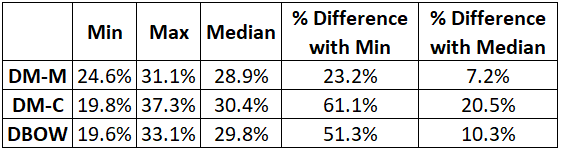
\includegraphics[width=0.48\textwidth]{infoRet-Cosine.png}
\end{figure}

\begin{figure}[ht]
\caption{Summary of Information Retrieval Results - Euclidean Distance}
\label{results_of_information_retrieval_euclidean}
\centering
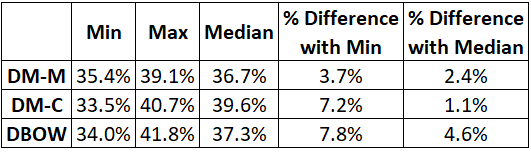
\includegraphics[width=0.48\textwidth]{infoRet-Euclidean.png}
\end{figure}

Using cosine similarity to determine if the two posts from the same tag were more similar in vector space than the other was expected to produce results with a lower rate of error, however, the Euclidean distance consistently outperformed.  ----FIGURES---  Figures 3 and 4 display the summaries of the results for cosine simularity and Euclidean distance respectively among all the datasets. The percentages were calculated from the fraction of correctly categorized posts such that the two posts from the same tag were deamed closer together in vector space, out of the total amount of times the model was tested. Highlights of the tests are as follows:

\begin{itemize}
  \item DM-M was the most consistent with both measurements among all three models. 
  \item Optimized DM-C was the most accurate model with Euclidean distance.
  \item Optimized DM-M was the most accurate model with cosine simularity and cose to DM-C with Euclidean distance.
  \item DBOW was the least accurate, but the fastest model to train. With proper optimization, it could be an alternative to datasets that are too large for DM.
  \item Feature vector size of 100 produced similar results to 300 size at 20 epochs, but was much faster and might be able to save time without sacrificing precision, however, 100 feature size with 50 epochs performed worse.
  \item Raising the minimum word count may help DM-C.
  \item Not every dataset generated the same correlation between parameter changes. Optimization depends on the individual dataset as well as the model type being used.
\end{itemize}

Overall, the default model of 300 feature vector size, 20 epochs, minimum word count of 1, total window size of 10, and negative set to 10 in DBOW performed well. DBOW and DM-C exhibited the ability to perform more accurately with optimizing of parameters, but not every dataset was impacted in the same way for one parameter change. For example, the highest percentage of correctly categorized posts in DM-C was brought on by increasing the 300 vector size model from 20 epochs to 50 in the just trained on python dataset, but the other two datasets suffered.

\subsubsection{Vector Prediction Analysis}

One can determine both how accurately and precie the model represents the trained data by generating an inferred vector from the training corpus and comparing it to the most similar learned vector from the model. If a document (stackoverflow post) is inferred to be the most similar to its trained self, then the model is an accurate representation of itself. If the model is largely accurate, but demonstrates a wide distribution of cosine simularity values, then the data may not be precise such that the posts differ greatly from one another.  ---FIGURE OF DATA FOR NORMAL, HIGH VECTOR, MORE EPOCHS, SMALL VECTOR----

Initially, testing was done on a dataset containing both python and javascript. To avoid taking the time to create special training datasets to be used against multiple combinations of parameters, data was not chosen randomly. All of the documents in a given training corpus were used during testing. The python and javascript dataset was the training dataset created randomly for information retrieval testing that contained 25,000 posts each from python and javascript.The results from initial information retrieval testing suggested that there was not a semantic differece between python and javascript posts so python was also tested alone with all parsed python posts (slightly less than 50,000). Since training the Doc2Vec models was hardware and time intensive, the database tag dataset was not tested as throughly as the python and javascript and just python datasets. The vector prediction analysis results of c\# and .net indicated they were not much different than just python so they were not tested further.  

The results revealed several interesting possibilities regarding the stackoverflow data:

-Models as a whole performec better with small 100 size feature vector. ---mostly decided by DM-C. DM-M worse. Both in python and javascript. 1st quartile and mean in DBOW very high

-DM-M performed the best with larger vectors, training more did not affect DM-M that much compared to vector size and window size. TEST 300v 20 epochs, 10 window, 50 epochs. better than window 16 at 50 epochs? 
-DM-M semi-consistent. 1-3.5 percent error. Combinining the paragraph vectors as suggested by Mikolov et all of DM-M and DBOW probably produce most consistent model good for data already trained and data that has not been seen - DM-M better at picking out topics  --> info RET.

-DM-C has the best Max when the vector was the largest - 400 neurons. More epochs ruined percent erro? TEST ABOVE. or was it the large 16 window? TEST 400v, 20epochs. best percent error when vector was small. Smaller vector = smaller vector space = less ability to determine semantic differences = better results if there is no relationship? -DBOW most consistent at percent error. Never broke .1. Good at predicting data that was already trained. Model based on probability distributions of words.
-DM-C has highest possibility for success, high maxes, but very large range, low Mins, wide 1st-3rd quartiles, low means. Probably does the best with very close semantic relationships as Mikolov suggested. They also used a combination of Dm-C and DBOW for better results. Very slow to train and did the worst with our sparce unrelated data so not worth it for this data.


-DBOW better in PYJS than just PY by .01-.02 . 20, 50-epochs not must difference. lowest at 300V 10 negative. still lower percent error than the others at other parameter changes. Consistently the best. Similar mean , quartile distribution as python. small difference between mean 1st and 3rd quartiles.


-the higher the epochs, the closer the 3rd quartile was to the max. Distance from 3rd quartile to 1st not greatly affected. Even though the percent erros would go down up with more epochs, the cosine simularities got better. Better the cosine simularity, the better the data is being represented by the model, better the topics can probably be dinstinguished? Some of the data must be very different semantically. Posts from untold amount of users on stackoverflow. 





 


\subsubsection{Conclusions}

some py > PyDb, PyJs , so training model on one thing might be better, especially when one topic like Js has lower correlation
Precision in vector prediction analysis was thought to affect info ret results, but it really didn't. New data very different than old.
Since DM-C depends on strong semantic relationships, a high error rate while measuring cosine simularity demonstrates a week semantic relationship between the individual stackoverflow tags. If the tags do not actually possess a semantic relationship, than 

A high error rate when trying to distinguish between topics suggests that there may be no actual semantic relationship between the stackoverflow data. Part of the problem might be the topics themselves. Python and javascript, for example, are both computer programming languages. Although they have different uses and purposes, the concepts surrounding them are more similar than say a programming language and more distance subject such as biology. To increase the semantic relationship, the stackoverflow data could be parsed more effectively. The data consisted of the 'posts' from stackoverflow. These posts did not contain the post titles or the comments. Both the titles and comment so often contain the most helpful information relevant to the topic at hand. 

Content with more specific information that is better suited for parsing could also be adopted instead. For example, typo-less information or cleaned up code from scholarly resources might allow for more efficient tokenization of relevant words or symbols like parathensis and brackets which are more prevalent in some programming languages than others. It is possible, however, that because the data from stack overflow comes from an untold amount of users, a semantic relationship may not be able to be determined. 

!!!Doc2Vec was not found to be successfull at predicting topics because of a lack of semantic relationships between datasets. Could be used to find already trained on and labeled data (VPA results) ------ If the model was accurate, could be used on pre-labeled trained data to suggest the labels from the most similar document to the inferred vector of the document being compared  --> Put in last papaer conclusion !!!!

\subsection{Evaluating Application}
\paragraph{Pre-Surveying}
To evaluate our project idea, we conducted a pre-surveying to see what the problem we are facing and how people reacting about our proposed solution. We asked our participants how long they will spend on find the right textbook, what aspect do they think is most important when choosing a textbook (except the content, our learning model will do the best of this part). See Table \ref{Pre-survey} for a breakdown of the questions to ask.
\begin{table}[!htbp]
\caption{\bf Questions in Pre-Survey} 
\label{Pre-survey}
\begin{center}
\begin{tabular}{  l  p{6cm} }
\bf NO & \bf QUESTIONS\\ \hline \\
1 & Are you a student or professor?\\
2 & How much time do you spend on choosing a textbook?\\
3 & How do you choose a textbook?\\
4 & What aspect do you think is most important when choosing a textbook (except the content)? \\
5 & Would you consider an app that will give you recommended textbooks base on your course syllabus and your preference? \\
\end{tabular} 
\end{center}
\end{table}
Among the 29 responses, we found that 73.3\% responded as they interested to our application to recommend the textbooks. The answer to most important aspect during the textbook chosen, review/ratings and sell price were the highest concern. These preliminary results give us the guidance to design the application and to improve the core learning models. See Figure \ref{result_of_presurvey} for detailed results.

\begin{figure}[ht]
\caption{Summary of Pre-survey}
\label{result_of_presurvey}
\centering
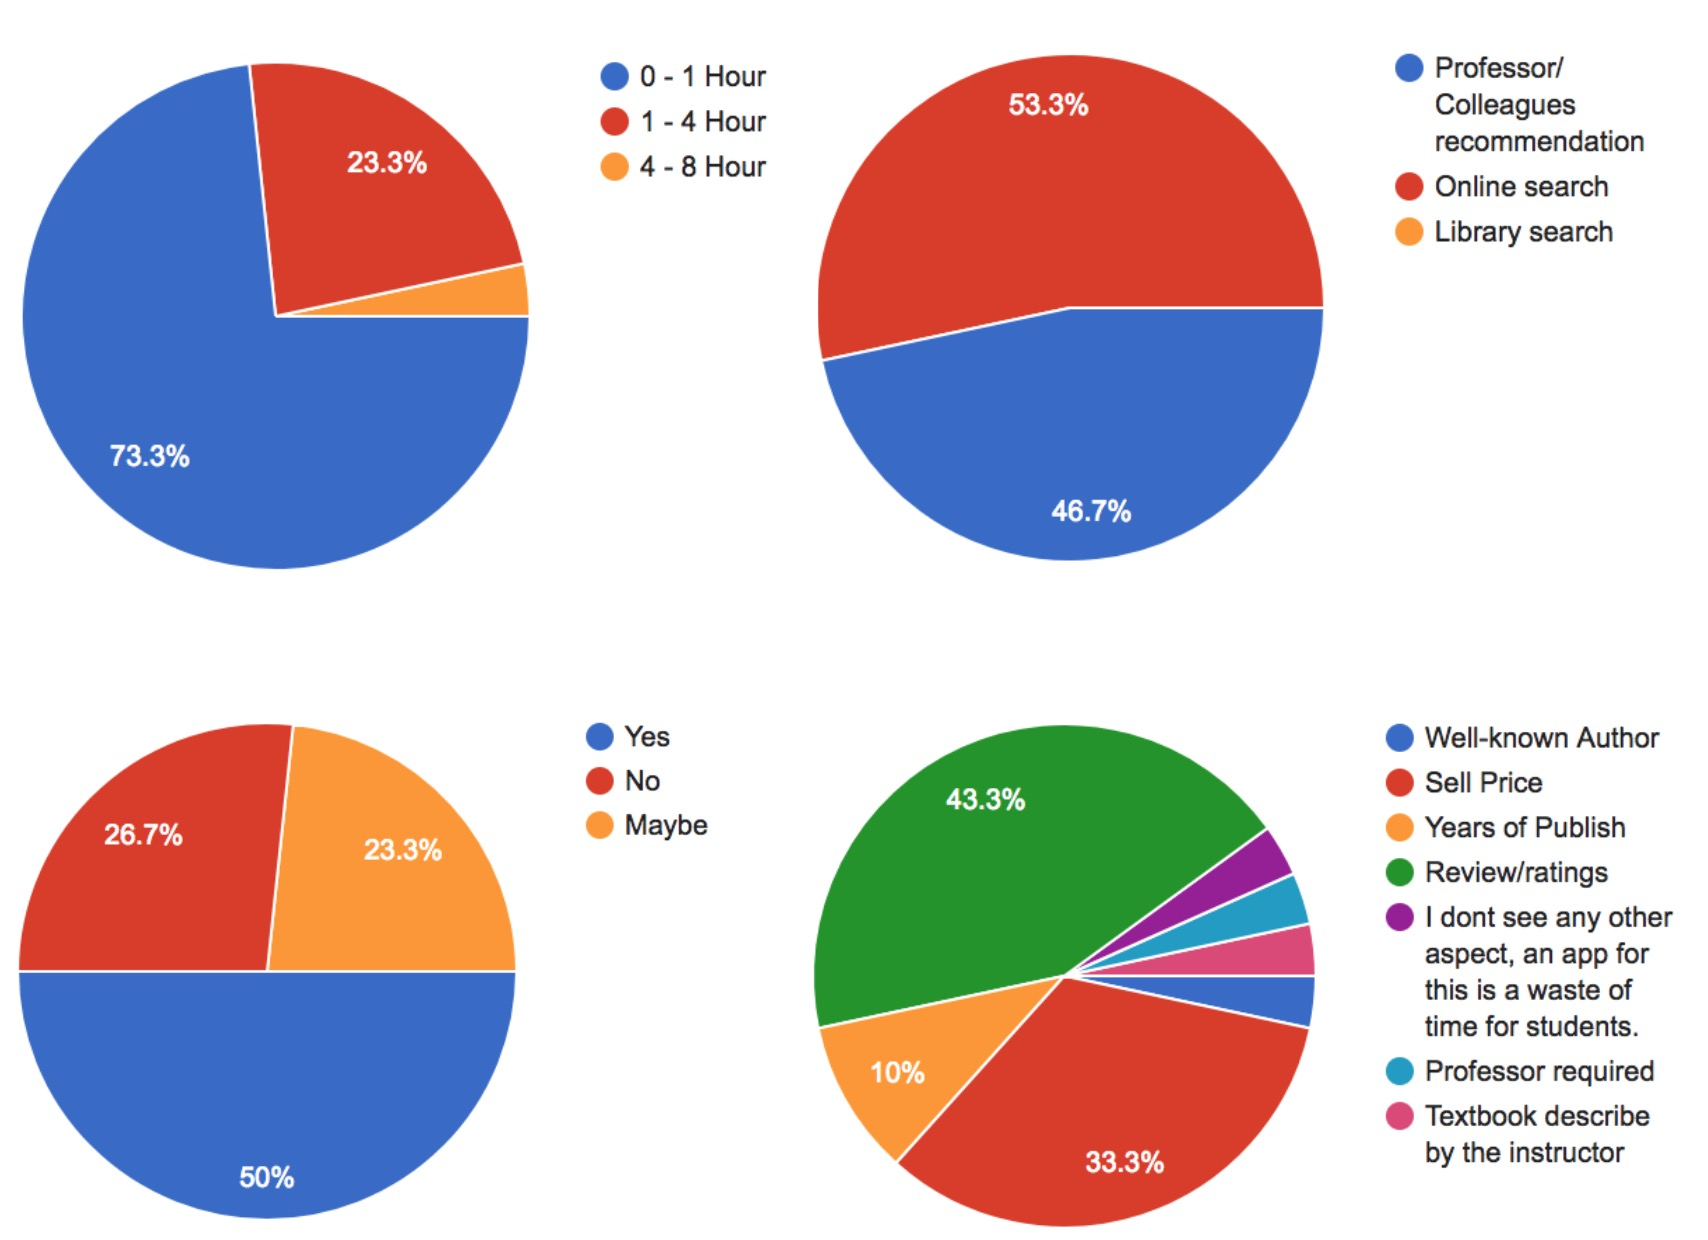
\includegraphics[width=0.5\textwidth]{preSurvey.jpeg}
\end{figure}

\paragraph{Experiments and Post-survey}
After we build the application with the command line interface and core learning models, we ran the experiments with different users in a focus group to evaluate the solution. We present our work to our peers to evaluate, after they try our application, we used google form to collect their opinions and comments on our application. Table \ref{post-survey} is the breakdown of the survey questions.
\begin{table}[!htbp]
\caption{\bf Questions in Post-Survey} 
\label{post-survey}
\begin{center}
\begin{tabular}{  l  p{6cm} }
\bf NO & \bf QUESTIONS\\ \hline \\
1 & I was able to run the test code (python analysis.py --verbose) with the documentation provided.\\
2 & I was unable to understand the structure of the code.\\
3 & What would you change about this CLI?\\
4 & What would scare you about working on this program or the resulting webapp?\\
5 & What do you like about this CLI? \\
6 & Commnets
\end{tabular} 
\end{center}
\end{table}

%%% Local Variables:
%%% mode: latex
%%% TeX-master: "../../main"
%%% End:
